\chapauth{King Plum the Nth}
\chapter{Flow My Tears, the PI Said.}


The kids from the neighborhood pooled their money to hire me. All
the kids on that street in the Bronx, in New York. One slow day I
was getting ready to leave the office a bit early when a kid pushed
open the door with my name, Luke Bavarious, and my job, private
detective, painted in neat black letters on the gray pebbled
glass.



``Mr.\ Bavarious?'' he said.

``That's what it says on the door, kid.'' He looked
like he was about 12.

``My friends and I need to hire a private detective to find
Mikey.'' He walked across the room trying to look brave,
shoved a hand in his jeans pocket, pulled out a wad of crumpled
\$5's and \$10's, and set them on my desk.



I eyed the dough suspiciously. It looked sticky and damp. I
can't remember ever not wanting to touch money before. I
reached out gently and poked at it. Maybe \$45 bucks. Maybe less. It
wasn't enough to pay for the time it'd take me to take
a piss all over their sorry case. Whatever it was.



``Your mother know you're here, kid?''

``Mister, Mikey's been missing, and all our parents and
the cops say he ran away, but we know he got taken.''

``Taken by what, kid?''

``Taken by a nameless horror, sir.''



I looked at the dough again. ``I charge a hundred and fifty an
hour, kid. In this traffic it'd cost ya another two fifty
five just to get me to set foot in the Bronx.'' The kid looked
like he was going to cry. I swore under my breath, stood, and
grabbed the cash from my desk. Shoving it into my pocket I said,
``Never mind. I'll bill this Mikey's folks for the
difference if I find him alive.'' The kid started sobbing
then. Really hard. While he got it out of his system, I opened my
desk drawer, pulled out my trusty Beretta and checked the
magazine.



Once I got to the Bronx it didn't take me long to find out
what had happened. Sometimes my job calls on me to fight monsters
of a supernatural nature. Sometimes I find myself buried neck deep
in the blackest culture, the world of the gothic and occult. But
sometimes the monsters are more horrible than monsters because
sometimes the monsters are men. And this monster was a man. He was
a homeless pedophile. Mikey wasn't his first but, by god, he
was going to be the last. I pulled my revolver and pointed it at
him,



``This is the end of the line, hobo.''

``You won't kill me, Bavarious! I used to be a cop. Like
your father. It's against the law to kill me no matter how
many kids I raped and killed.''

He had me. I knew, and he know, and my father --- god rest him
--- had known, no matter how many kids you rape and kill it
only warrants murder in certain states and then only after a
lengthy judiciary process. But, looking at poor Mikey's
broken, rotten corpse, I just wasn't sure if any of that
really mattered.



The sick hobo followed my gaze to the body of his most recent
victim.



``Oh, him? Don't worry about him. He liked
it.''



And that's when I snapped. Everything became crystal clear. I
wasn't sure what was right or wrong anymore but there was one
thing I knew for damn sure. Mikey didn't like it.



I pulled my trigger. My Beretta belched hot lead. The shell hitting
the warehouse floor made a sound like a polite cough afterward. A
ragged, bloody hole exploded in the monster's gut. He
stopped, stared at his gory wound and began to vomit. Vomit flowed
from his mouth and, after a second, shot from the bullet wound in
his stomach too. I pulled the trigger again and again, each time it
was less for anger and more for mercy. I perforated his neck. He
kept vomiting. The vomit flowed from his mouth and gut and the hole
in his neck. I put a hole in his head --- right between the
eyes --- his eyes crossed looking up trying to see his death
wound. His body heaved again and again, and vomit poured from his
forehead too. Torrents of blood and bile and breakfast pouring from
four holes on his body, three of them man made.



Finally, I could take it no more, my stomach surrendered and I
vomited. As I vomited, my eyes slipped back to the body of the
monster's latest victim and I wept and my tears commingled
with the vomit. There we stood, the two of us, vomiting. The psudo
mythical hero and the psudo mythical monster over the poor broken
body that had so recently vomited a child's soul into the
afterlife. In a way, we were brothers, in vomit. He fell to his
knees. He died. And, although I stopped vomiting, eventually, I
could not stop sobbing. I cried so hard the flow of my tears washed
the vomit away. 
 






\begin{figure}[b]
  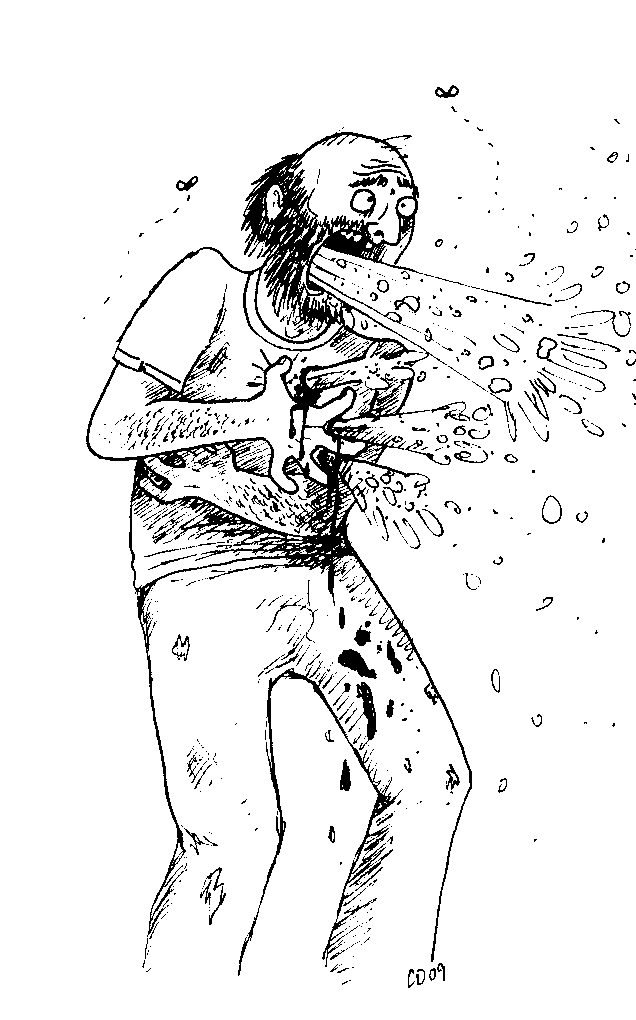
\includegraphics[width=\textwidth]{art/Part_of_Everything-Bullet_Barf.png}
  \caption{Artwork by Part of Everything}
\end{figure}
